%!TEX root = ../main.tex

\section{Problem Formulation}
\label{section:focus-problem-definition}

A \emph{counterfactual explanation} for an instance $x$ and a model $f$, $\Delta_{x}$, is a minimal perturbation of $x$ that changes the prediction of $f$. 
$f$ is a probabilistic classifier, where $f(y\mid x)$ is the probability of $x$ belonging to class $y$ according to $f$.
The prediction of $f$ for $x$ is the most probable class label $y_x = \arg\max_{y} f(y \mid x)$, and
a perturbation $\bar{x}$ is a counterfactual example for $x$ if, and only if, $y_x \not = y_{\bar{x}}$, that is:
%
\begin{align}
\arg\max_{y} f(y \mid x)
\not =
\arg\max_{y'} f(y' \mid \bar{x}).
\label{eq:cfexample}
\end{align}
%
In addition to changing the prediction, the distance between $x$ and $\bar{x}$ should also be minimized. 
We therefore define an \emph{optimal counterfactual example} $\bar{x}^*$ as: 
\begin{equation}
 \bar{x}^* := \arg\min_{\bar{x}} d(x, \bar{x}) 
 \text{ such that }
y_x \not = y_{\bar{x}},
\label{eq:optimalcondition}
\end{equation}
\noindent
where $d(x, \bar{x})$ is a differentiable distance function. 
The corresponding \emph{optimal counterfactual explanation} $\Delta^*_{x}$ is:
\begin{align}
\Delta^*_{x} = \bar{x}^* - x.
\end{align} 
%\begin{align}
%\begin{split}
% \bar{x}^*&{} := \arg\min_{\bar{x}} d(x, \bar{x})  \\
%& \text{such that }
%\arg\max_{y} f(y \mid x)
%\not =
%\arg\max_{y} f(y \mid \bar{x}).
%\end{split}
%\label{eq:optimalcondition}
%\end{align}
%\todo{It would be nice to better place this in the field, i.e. cite people who agree/disagree with this definition.}
This definition aligns with previous ML work on counterfactual explanations \citep{laugel_inverse_2017, karimi_model-agnostic_2019, tolomei_interpretable_2017}. 
We note that this notion of \emph{optimality} is purely from an algorithmic perspective and does not necessarily translate to optimal changes in the real world, since the latter are dependent on the context in which they are applied. 
It should be noted that if the loss space is non-convex, it is possible that more than one optimal counterfactual explanation exists.

Minimizing the distance between $x$ and $\bar{x}$ should ensure that $\bar{x}$ is as close to the decision boundary as possible. 
This distance indicates the effort it takes to apply the perturbation in practice, and an optimal counterfactual explanation shows how a prediction can be changed with the least amount of effort.
An optimal explanation provides the user with interpretable and potentially actionable feedback related to understanding the predictions of model $f$. 


\citet{wachter_counterfactual_2017} recognized that counterfactual examples can be found through gradient descent if the task is cast as an optimization problem.
Specifically, they use a loss consisting of two components: 
\begin{enumerate*}[label=(\roman*)]
%	\item a prediction loss to change the prediction of $f$: $\mathcal{L}_{pred}(y_x, \bar{x} \mid f)$, and
	\item a prediction loss to change the prediction of $f$: $\mathcal{L}_{pred}(x, \bar{x} \mid f)$, and
	\item a distance loss to minimize the distance $d$: $\mathcal{L}_{dist}(x, \bar{x} \mid d)$.
\end{enumerate*}
The complete loss is a linear combination of these two parts, with a weight $\beta \in \mathbb{R}_{>0}$:
\begin{align}
\label{eq:mainloss}
%\mathcal{L}(x, \bar{x} \mid f, d) = \mathcal{L}_{pred}(y_x, \bar{x} \mid f) + \beta \mathcal{L}_{dist}(x, \bar{x} \mid d), 
\mathcal{L}(x, \bar{x} \mid f, d) = \mathcal{L}_{pred}(x, \bar{x} \mid f) + \beta \mathcal{L}_{dist}(x, \bar{x} \mid d).
\end{align}
%where $y_x = \arg\max_{y} f(y \mid x)$ is the original predicted class according to $f$. 
The assumption here is that an optimal counterfactual example $\bar{x}^*$ can be found by minimizing the overall loss:
\begin{align}
\bar{x}^* = \arg\min_{\bar{x}} \mathcal{L}(x, \bar{x} \mid f, d).
\end{align}
\citet{wachter_counterfactual_2017} propose a prediction loss $\mathcal{L}_{pred}$ based on the mean-squared-error. 
A clear limitation of this approach is that it assumes $f$ is differentiable.
This excludes many commonly used ML models, including tree-based models, which we focus on in this work.


\section{Method: FOCUS}
\label{section:focus-method}
To mimic many real-world scenarios, we assume there exists a trained model $f$ that we need to explain. The goal here is not to create a new, inherently interpretable tree-based model, but rather to explain a model that already exists. 


\subsection{Loss Function Definitions}

We use a hinge-loss since we assume a classification task:
%
\begin{align}
\mathcal{L}_{pred}(x, \bar{x} \mid f) = {\mathbbm{1}}\left[\arg\max_{y} f(y \mid x) = \arg\max_{y'} f(y' \mid \bar{x})\right] \cdot  f(y' \mid \bar{x}).
\end{align}
%
Allowing for flexibility in the choice of distance function allows us to tailor the explanations to the end-users' needs. We make the preferred notion of \emph{minimality} explicit through the choice of distance function. 
Given a differentiable distance function $d$, the distance loss is: 
%
\begin{align}
\mathcal{L}_{dist}(x, \bar{x}) = d(x, \bar{x}). 
\end{align}
%
Building off of \citet{wachter_counterfactual_2017}, we propose incorporating differentiable approximations of non-differentiable models to use in the gradient-based optimization framework. 
Since the approximation $\tilde{f}$ is derived from the original model $f$, it should match $f$ closely: $\tilde{f}(y \mid x) \approx f(y \mid x)$. 
We define the approximate prediction loss as follows:
\begin{align}
\widetilde{\mathcal{L}}_{pred}(x, \bar{x} \mid f, \tilde{f}) = \mathbbm{1}\left[\arg\max_{y} f(y \mid x) = \arg\max_{y'} f(y' \mid \bar{x})\right] \cdot  \tilde{f}(y' \mid \bar{x}).
\end{align}
This loss is based both on the original model $f$ and the approximation $\tilde{f}$:
the loss is active as long as the prediction according to $f$ has not changed, but its gradient is based on the differentiable $\tilde{f}$. 
This prediction loss encourages the perturbation to have a different prediction than the original instance by penalizing an unchanged instance. 
The approximation of the complete loss becomes:
\begin{equation}
\widetilde{\mathcal{L}}(x, \bar{x} \mid f, \tilde{f}, d) =\widetilde{\mathcal{L}}_{pred}(x, \bar{x} \mid f, \tilde{f}) + \beta \cdot \mathcal{L}_{dist}(x, \bar{x} \mid d).
\label{eq:approxloss}
\end{equation}
Since we assume that it approximates the complete loss, 
\begin{align}
\widetilde{\mathcal{L}}(x, \bar{x} \mid f, \tilde{f}, d) \approx \mathcal{L}(x, \bar{x} \mid f, d),
\end{align}
we also assume that an optimal counterfactual example can be found by minimizing it:
%
\begin{align}
\bar{x}^* \approx \arg\min_{\bar{x}} \, \widetilde{\mathcal{L}}(x, \bar{x} \mid f, \tilde{f}, d).
\label{eq:xbar}
\end{align}

\begin{figure}[t]
\centering
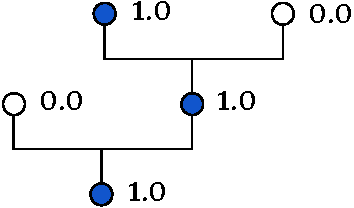
\includegraphics[scale=0.7]{04-research-focus/figures/real_tree} 
\quad
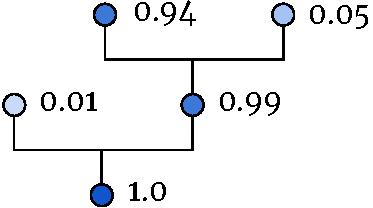
\includegraphics[scale=0.7]{04-research-focus/figures/approx_tree}
\vspace{2mm}
\caption{
Left: A decision tree $\mathcal{T}$ and node activations for a single instance. Right: a differentiable approximation of the same tree $\widetilde{\mathcal{T}}$ and activations for the same instance.
}
\label{fig:exampletrees}
\end{figure}


\subsection{Tree-based Models}
To obtain the differentiable approximation $\tilde{f}$ of $f$, we construct a probabilistic approximation of the original tree ensemble $f$.
Tree ensembles are based on decision trees; a single decision tree $\mathcal{T}$ uses a binary-tree structure to make predictions about an instance $x$ based on its features.
Figure~\ref{fig:exampletrees} shows a simple decision tree consisting of five nodes.
A node $j$ is activated if its parent node $p_j$ is activated and feature $x_{f_j}$ is on the correct side of the threshold $\theta_j$; which side is the correct side depends on whether $j$ is a \emph{left} or \emph{right} child. 
The root note is an exception, it is always activated.
Let $t_j(x)$ indicate if node $j$ is activated:
\begin{equation}
\mbox{}\hspace*{-2mm}t_j(x) =
    \begin{cases}
   1, & \text{if $j$ is the root}, \\
   t_{p_j}(x) \cdot  \mathbbm{1}[x_{f_j} > \theta_j], & \text{if $j$ is a left child}, \\
    t_{p_j}(x) \cdot  \mathbbm{1}[x_{f_j} \leq \theta_j], &\text{if $j$ is a right child}.
    \end{cases}
\end{equation}
$\forall x, \,  t_0(x) = 1$.
Nodes that have no children are called \emph{leaf nodes}; an instance $x$ always ends up in a single leaf node.
Every leaf node $j$ has its own predicted distribution $\mathcal{T}(y \mid j)$; the prediction of the full tree is given by its activated leaf node. 
Let $\mathcal{T}_{\textit{leaf}}$ be the set of leaf nodes in $\mathcal{T}$, then:
\begin{equation}
(j \in \mathcal{T}_{\textit{leaf}} \land t_j(x) = 1) \rightarrow \mathcal{T}(y \mid x) = \mathcal{T}(y \mid j).
\end{equation}
Alternatively, we can reformulate this as a sum over leaves:
\begin{equation}
\mathcal{T}(y \mid x) = \sum_{j \in \mathcal{T}_\mathit{leaf}}  t_j(x) \cdot \mathcal{T}(y \mid j).
\end{equation}
Generally, tree ensembles are deterministic; let $f$ be an ensemble of $M$ many trees with weights $\omega_m \in \mathbb{R}$, then:
\begin{equation}
f(y \mid x)
=  \arg\max_{y'} \sum_{m=1}^M \omega_m \cdot \mathcal{T}_m(y' \mid x).
\end{equation}


\subsection{Approximations of Tree-based Models}
If $f$ is not differentiable, we are unable to calculate its gradient with respect to the input $x$. 
However, the non-differentiable operations in our formulation are 
\begin{enumerate*}[label=(\roman*)]
	\item the indicator function, and
	\item a maximum operation, 
\end{enumerate*}
both of which can be approximated by differentiable functions.
First, we introduce the $\widetilde{t}_j(x)$ function that \emph{approximates the activation of node} $j$: $\widetilde{t}_j(x) \approx t_j(x)$, using a sigmoid function with parameter $\sigma \in \mathbb{R}_{>0}$:
$
\textit{sig}(z) = (1 + \exp(\sigma \cdot z))^{-1}
$
and
\begin{align}
\widetilde{t}_j(x) &{} =
    \begin{cases}
    1, & \text{if $j$ is the root}, \\
   \widetilde{t}_{p_j}(x) \cdot \textit{sig}(\theta_j {-} x_{f_j}), & \text{if $j$ is left child}, \\
   \widetilde{t}_{p_j}(x) \cdot  \textit{sig}( x_{f_j} {-} \theta_j), & \text{if $j$ is right child}.
    \end{cases}
\label{eq:sigma}    
\end{align}
As $\sigma$ increases, $\widetilde{t}_j$ approximates $t_j$ more closely.
Next, we introduce a \emph{tree approximation}:
\begin{equation}
\widetilde{\mathcal{T}}(y \mid x) = \sum_{j \in \mathcal{T}_\mathit{leaf}}  \widetilde{t}_j(x) \cdot \mathcal{T}(y \mid j).
\end{equation}
The approximation $\widetilde{\mathcal{T}}$ uses the same tree structure and thresholds as $\mathcal{T}$.
However, its activations are no longer deterministic but instead are dependent on the distance between the feature values $x_{f_j}$ and the thresholds $\theta_j$.
Lastly, we replace the maximum operation of $f$ by a softmax with temperature $\tau\in\mathbb{R}_{>0}$, resulting in:
\begin{align}
\tilde{f}(y \mid x)
= \frac{
\exp\left(\tau \cdot \sum_{m=1}^M \omega_m \cdot \widetilde{\mathcal{T}}_m(y \mid x)\right)
}{
\sum_{y'} \exp\left(\tau \cdot \sum_{m=1}^M \omega_m \cdot \widetilde{\mathcal{T}}_m(y' \mid x)\right)
}.
\label{eq:tau}
\end{align}
The approximation $\tilde{f}$ is based on the original model $f$ and the parameters $\sigma$ and $\tau$.
This approximation is applicable to any tree-based model, and 
how well $\tilde{f}$ approximates $f$ depends on the choice of $\sigma$ and $\tau$.
The approximation is potentially perfect since
\begin{align}
\lim_{\sigma,\tau\rightarrow\infty}
\tilde{f}(y \mid x) = f(y \mid x).
\end{align}
%
\subsection{Our Method: FOCUS}
We call our method FOCUS: Flexible Optimizable CounterfactUal Explanations for Tree EnsembleS. 
It takes as input an instance $x$, a tree-based classifier $f$, and two hyperparameters: $\sigma$ and $\tau$, which we use to create the approximation $\tilde{f}$. 
Following Equation~\ref{eq:xbar}, FOCUS outputs the optimal counterfactual example $\bar{x}^*$, from which we derive the optimal counterfactual explanation $\Delta^*_{x} = \bar{x}^* - x$. 
%\mdr{Now introduce the FOCUS acronym and say what the method is, including what the inputs and outputs of the method are.}

\subsection{Effects of Hyperparameters}
Increasing $\sigma$ in $\tilde{f}$ eventually leads to exact approximations of the indicator functions, while increasing $\tau$ in $\tilde{f}$ leads to a completely unimodal softmax distribution. 
It should be noted that our approximation $\tilde{f}$ is not intended to replace the original model $f$ but rather to create a differentiable version of $f$ from which we can generate counterfactual examples through optimization. 
In practice, the original model $f$ would still be used to make predictions and the approximation would solely be used to generate counterfactual examples. 
